\documentclass{article}

\usepackage{ucs} % Unicode - dependency of utf8x inputenc
\usepackage[utf8x]{inputenc} % "utf8x" uses "ucs"-package, better than "UTF8"
\usepackage[T1]{fontenc}
\usepackage{lmodern}

\usepackage[english]{babel}
\usepackage{amsmath, amssymb, amsxtra, amsthm}
\usepackage{epsfig,psfrag}
\usepackage{listings}
\usepackage{url}

\usepackage{epstopdf}

\usepackage[table]{xcolor}
\usepackage{tikz}

\usepackage{nicefrac}
\usepackage[toc,page]{appendix}


\theoremstyle{definition}
\newtheorem*{example}{Example}

\newcommand{\refchapter}[1]{Chapter~\ref{#1}}
\newcommand{\refsec}[1]{Section~\ref{#1}}
\newcommand{\refeqn}[1]{Equation~(\ref{#1})}
\newcommand{\reffig}[1]{Figure~\ref{#1}}
\newcommand{\reftbl}[1]{Table~\ref{#1}}

\title{
{\bf \scriptsize RHEINISCH-WESTF\"ALISCHE TECHNISCHE HOCHSCHULE AACHEN \\
LuFG Informatik 12 (Prof. Dr. rer. nat. Uwe Naumann)}
\vspace{.5cm} \\
\epsfig{file=figures/STCE_Logo_WWW.eps,width=.7\textwidth}
\vspace{1cm} \\
{\bf \Large Numerical Libraries} \\
{\bf \large Statistics} \\
{\large The $\chi^2$ and Kolmogorov-Smirnov tests in the NAG C Library}
}

\author{Christian Janßen (302530) \\ Fabian Ohler (280424) }
\date{July 15, 2013}

\begin{document}

\lstloadlanguages{[ISO]C++, R}
\lstset{basicstyle=\small, numbers=left, numberstyle=\footnotesize, tabsize=2,
  stepnumber=1, numbersep=5pt, breaklines=true, escapeinside={/*@}{@*/}}

\begin{titlepage}
\clearpage
\maketitle
\thispagestyle{empty}
\end{titlepage}

\section*{Erkl\"arung}

Hiermit versichere ich, dass ich die Arbeit selbst\"andig verfasst und keine
anderen als die angegebenen Quellen und Hilfsmittel benutzt sowie Zitate 
kenntlich gemacht habe.
\\
\vspace{10ex}
\\
Ort, Datum \hfill Ort, Datum
\\
\vspace{10ex}
\\
Christian Janßen \hfill Fabian Ohler

\newpage

\tableofcontents

\pagestyle{headings}
\newpage

\section{Introduction}
Statistics as a part of mathematics describes collecting, evaluating and judging of informations and data. In addition it serves the stochastic as a connection between empirical datasets and their respective hypothesis. Those datasets help prognosticating future events like the daily weather forecast.The Statistics helps to create hypotheses explaining the distribution of values of discrete datasets and this allowing conclusions about areas where no data is provided. This is useful for example while calculating TV ratings on basis of a few observed television viewers.\\
Due to the obvious fact that not all hypotheses are qualified for a specific dataset, these hypotheses must be checked in terms of correctness and precision.
The better the precision of a hypothesis or its ability to explain a dataset the better is its goodness of fit.
The checks to measure the quality of hypotheses is done by ``goodness of fit'' tests. Since such tests need all empirical data gathered and the calculation of distribution functions to evaluate a hypothesis, they are normally to time consuming to do it manually. To speed up and automate the procedure of execution of ``goodness of fit'' tests there exists various numerical libraries.\\ 
In this written elaboration the $\chi^2$ and the ``Kolmogorv-Smirnov'' tests is presented with their implementation in the numerical library ``NAG C'' together with another alternative library. Between various alternatives such as R \cite{hellbrueck2009angewandte}, Matlab \cite{benker2001statistik}, and Mathematica \cite{jaeger1997statistik}, we decided to present the test equivalents in R, as it on its way to being the most commonly used language for statistical applications and all comparable major applications provide interfaces to it.
\section{Basic Statistics}
This section is intended to provide the basic knowledge about statistics up to statistical hypothesis testing needed to understand the two algorithms this paper focuses on.

\subsection{Fundamentals}
As the goal is to understand tests on hypothesis, we place an emphasis on experiments.
When conducting an experiment, different outcomes are possible, otherwise it would make little sense to do so.
The collection of all possible outcomes of an experiment shall be called \emph{sample space}.
Analogue a possible outcome is called a \emph{point in the sample space}.
Now we can define the omnipresent term \emph{event} as any set of points in the sample space.
One is usually interested in the \emph{probability of an event A}, denoted by P(A).
To determine those, we need a \emph{probability function}, assigning real numbers to points in the sample space.
The terms introduced shall now be illustrated using an example.
\begin{example}[Flipping a coin \cite{conover1980practical}]
	We conduct the following experiment:
	A fair coin is flipped twice and the outcome is denoted by T for tails and H for heads.
	Our sample space is the set \{TT, TH, HT, HH\}.
	The event `at least one head' includes the following points in the sample space: HT, TH, HH.
	As every point in the sample space is equally likely, our probability function assigns the same value to each of them (0.25).
	The probability of the event `at least one head' is 0.75.
\end{example}
Furthermore we define the term \emph{random variable}, meaning a function assigning real numbers to points in the sample space.
In contrast to the probability function the random variable acts as an enumerator.
The \emph{probability function of a random variable} X (denoted by $f(x)$) gives the probability of X assuming a point in the sample space, that X assigns the number x, so $f(x) = P(X = x)$, where $X = x$ is an event the probability function $P$ gives a probability for.
A \emph{cumulative distribution function $F(x)$ of a random variable} X gives the probability of X being less than or equal to x, formalized as: $F(x) = P(X \leq x) = \sum_{t\leq x}f(t)$.
Quantiles $x_p$ for probabilities $p$ mark the points in the sample space with $P(X<x_p)\leq p$ and $P(X>x_p)\leq 1-p$.
E.\,g. the 0.5th quantile $x_{0.5}$ divides the sample space into two halves and is also called median.
The \emph{expected value of a real valued function} $u(X)$ of a random variable X with the probability function $f(x)$ is denoted by $E[u(X)] = \sum_{x}u(x)f(x)$.
The well known \emph{mean of a random variable X} can then be written as $\mu = E(X) = \sum_{x}xf(x)$.
Analogue, we define the \emph{variance of a random variable X} with mean $\mu$ and probability function $f(x)$ as $\sigma^2 = E[(X-\mu)^2]$ and its positive square root as the \emph{standard deviation}, denoted by $\sigma$.

\subsection{Probability Distributions}
Later on, we want to test, whether or not a sample may obey a specific distribution function.
Therefore we now present some of the common distribution functions.
\\
The most simple distribution is the \emph{uniform distribution}, usually denoted by $\mathcal{U}(a,b)$ with $a$ and $b$ being the minimum and maximum values, respectively.
Its cumulative distribution function is given by 
\begin{equation}
F(x) = \left\{\begin{tabular}{ll}
0 & for $x<a$ \\
$\frac{x-b}{b-a}$ & for $a\leq x<b$ \\
1 & for $x\geq b$ \\
\end{tabular}\right.
\end{equation}
%
With the \emph{binomial distribution} $B(n,p)$, the number of successes in $n$ independent experiments with a boolean result and a success probability $p$ for each of the experiments can be described.
Its cumulative distribution function is given by
\begin{equation}
F(x) = \sum_{i\leq x} \genfrac(){0pt}{}{n}{i} p^{i}q^{n-i}
\end{equation}
%
Another well known distribution is the \emph{normal distribution} $\mathcal{N}(\mu,\sigma^2)$, parameterized by its mean $\mu$ and variance $\sigma^2$.
With $\mu = 0$ and $\sigma = 1$ it is called the \emph{standard normal distribution}.
Its general cumulative distribution function is given by
\begin{equation}
F(x) = \Phi\left(\frac{x - \mu}{\sigma}\right) = \frac{1}{\sqrt{2\pi\sigma}} \int_{-\infty}^{x}e^{-\frac{1}{2}[(y-\mu)/\sigma]^2}\textrm{d}y
\end{equation}
%
A distribution of special interest for the focus of this paper is the \emph{chi squared distribution} $\chi^2(k)$.
It is parameterized by the \emph{degrees of freedom} $k$.
Its cumulative distribution function is given by
\begin{equation}
F(x) = \left\{\begin{tabular}{ll}
$\int_{0}^{x} \frac{y^{(k/2)-1}e^{(y/2)}}{2^{k/2}\Gamma(k/2)}\textrm{d}y$ & if $x>0$ \\
0 & if $x\leq 0$
\end{tabular}\right.
\end{equation}
\begin{example}[\cite{conover1980practical}]
Let $X_1, \ldots, X_k$ be $k$ independent and identically distributed standard normal random variables. Let $Y = \sum_{i=1}^{k}X_i^2$. Then $Y$ has the $\chi^2$ distribution with $k$ degrees of freedom.
\end{example}

\subsection{Estimation}
\begin{description}
	\item[population] all elements under investigation
	\item[sample] collection of some elements of a population
	\item[target population] population, one wants information about
	\item[sampled population] population, one has information about
	\item[random sample] a sample from a finite population is a random sample if each of the possible samples was equally likely to be obtained
	\item[random sample of size n] is a sequence of n independent and identically distributed random variables $X_1, \ldots, X_n$
\end{description}

estimates:
quality criteria of an estimate: precision (how close to the real value) and reliability (probability for the result to be correct)
point estimates: sample mean, sample variance, ...
confidence interval: consist of \emph{interval estimate} borders and the \emph{confidence coefficient} (probability, that the interval estimator will contain the unknown population quantity)

\begin{description}
	\item[empirical distribution function] Let $X_1, \ldots, X_n$ be a random sample. The empirical distribution function $S(x)$ is a function of $x$, which equals the fraction of $X_i$s that are less than or equal to $x$ for each $x$, $-\infty<x<\infty$.
	\item[sample mean] Let $X_1, \ldots, X_n$ be a random sample. $\overline{X} = \frac{1}{n}\sum_{i=1}^{n}X_i$ is the sample mean.
	\item[sample variance] Let $X_1, \ldots, X_n$ be a random sample. $S^2 = \frac{1}{n}\sum_{i=1}^{n}(X_i-\overline{X})$ is the sample variance. The positive square root of the sample variance is the sample standard deviation $S$.
\end{description}

\subsection{Statistical Inference}

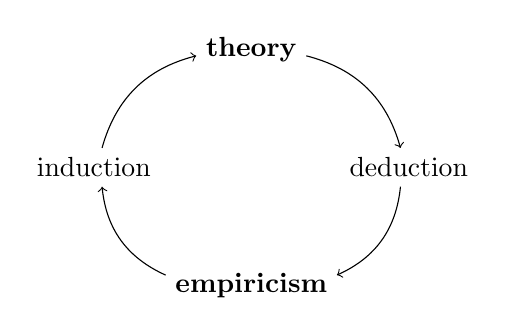
\begin{tikzpicture}[node distance = 2 cm]
	\node (t) at (2,3) {\bfseries theory};
	\node (d) at (4,1.5) {deduction};
	\node (i) at (0,1.5) {induction};
	\node (e) at (2,0) {\bfseries empiricism};
	\path
		(t) edge[bend left, ->] node[right] {} (d)
		(d) edge[bend left, ->] node[left] {} (e)
		(e) edge[bend left, ->] node[right] {} (i)
		(i) edge[bend left, ->] node[left] {} (t) ;
\end{tikzpicture}


hypothesis testing as a mean of statistical induction \\
process of inferring from a sample whether or not to accept a certain statement about the population \\
the statement itself has to be a hypothesis. \\
%
The word hypothesis may in this context be defined as
\begin{quote}
	a tentative assumption made in order to draw out and test its logical and empirical consequences \cite{merriamwebster}
\end{quote}
It can be seen as a more formal version of an \emph{educated guess}.
Using a hypothesis, one may predict e.\,g. the outcome of experiments.
Generally, a hypothesis is required to be either falsifiable or verifiable, such that it can be tested.


\subsection{Statistical Tests}
A statistical test performs a test on a hypothesis against the \emph{evidence} in a sample.
In the context of statistics, a hypothesis under test is often called the \emph{null hypothesis} ($H_0$) and its logical complement is called the \emph{alternative hypothesis} ($H_1$).
\\
When testing the null hypothesis, two answers can be given:
\begin{enumerate}
	\item $H_0$ is rejected
	\item $H_0$ is accepted
\end{enumerate}
The first answer states that $H_0$ is false and therefore $H_1$ is true.
Yet, the second answer only states that $H_0$ is not rejected, so it may or may not be true.
Sometimes, the literature gives three answer options \cite{weigand2009statistik}.
This is useful when looking at tests different than the ones focused on in this paper.
\\
With these answers at hand, we have to make a hypothesis the 
\\
The set of points in the sample space leading to the rejection of the null hypothesis is also called the critical region.
\\
It would be desirable for tests to always find the correct answer, but since we have to rely upon samples, there may be answers incorrect in the sense of the target population.
We distinguish between two types of errors when choosing an incorrect answer as in \cite{conover1980practical}:
\begin{description}
	\item[type I error] is the error of rejecting a true null hypothesis
	\item[type II error] is the error of accepting a false null hypothesis
\end{description}
The probability to commit a type I error is also called the \emph{significance level}, denoted by $\alpha$.
When denoting the probability to commit a type II error by $\beta$, the probability of rejecting a false null hypothesis is also called the \emph{power}, denoted by $1-\beta$.



\section{Kolmogorov–Smirnov Test}
In statistics the Kolmogorov-Smirnov-test is a nonparametric test which checks for equality of two probability distributions.
With this test one can check either if a given set of random samples follows a specified probability distribution or if two sets of random samples have the same probability distribution.\\
The first alternative is called ``one sample Kolmogorov-Smirnov-test'' and is a goodness of fit test. The ``two sample  Kolmogorov-Smirnov-test'' is the second alternative, but due to the limited space it will be neglected in this written elaboration.

\subsection{Mathematical Background}
In the following the proceeding of the execution of the goodness of fit test is described and will be later explained by means of an illustrative example. \\
For a random variable $X$ a set of $n$ observations ordered ascending such that $x_1 \le x_2 \le ... \le x_n$ is given. For those $n$ values the empirical distribution function $S(x)$  is determined.
The value of $S(x)$ for a given $x$ is just a simple counting of values which are less than or equal $x$ and then dividing this number by $n$. Formally written: 
$$S(x) = \frac{1}{n} \sum\limits^n_{i=1} I_{x_i\le x}~,$$
where $I_{x_i\le x}$ is the indicator function, which equals $1$ if $x_i\le x$ and equals $0$ if $x_i>x$.\\
After $S(x)$  is determined one has to formulate the null hypothesis 
$$H_0:S (x)=F_0 (x)~,$$ 
where $F_0 (x)$ is a manually chosen probability distribution.\\
The alternative hypothesis 
$$H_1:S (x)\ne F_0 (x)$$ 
means that the random variable does not follow the probability distribution $S(x)$.\\
The Kolmogorov-Smirnov test statistic is
$$D_n = \max (d_0,d_1)~,$$
where 
$$d_0=\max_{X} |S(x)-F(x)|$$ 
and
$$d_1 = \max_{x_i \in X} | S(x_{i-1})-F(x_i)|~,$$
with $S (x_0)$  defined as $0$. With a significance level $\alpha$, the value $D_n$ is then compared to a value $D_\alpha$~\cite{nagcKS}.
The value $D_\alpha$ is the critical value of the Kolmogorov distribution, which will not be discussed here, can be looked up in a table if $n$ is less than or equal $35$~\cite{massey1951}. If $n$ is greater than $35$, then the approximate value can be calculated with formulas found also in a table with respect to the chosen significance level~\cite{massey1951}. If $D_n>D_\alpha$ the null hypothesis $H_0$  is rejected at a significance level $\alpha$.

%\subsection{Mathematical Background}
\subsection{Example}
An illustrative example for the use of the ``one-sample-Kolmogorov-Smirnov-test'' is the following everyday situation.\\
While drinking a few wheat beer at the local pub, Paul and Franz start discussing about the height of the head of their beer.
Paul states that the head of his beer has a normal, average height, while Franz claims, the average height is normally higher.\\
Because they do not come to a conclusion, Franz takes out his measuring tape and measures the height of the heads and writes them down. Due to the obvious fact that two observations are not enough to give a statement about the average height, they order few more wheat beer, measure the height from every beer head and write it down.
After rearranging the observations into an ascending order, the following table is obtained:
\begin{table}[h]
\center
\begin{tabular}{c|c|c|c|c|c|c|c|c|c}
$x_1$	&$x_2$	&$x_3$	&$x_4$	&$x_5$	&$x_6$	&$x_7$	&$x_8$	&$x_9$	&$x_{10}$\\
\hline
1	&1.1	&1.2	&1.6	&1.7	&2.1	&2.1	&2.4	&2.4	&2.5	\\
\end{tabular}
\begin{tabular}{c|c|c|c|c|c|c|c|c|c}
$x_{11}$	&$x_{12}$	&$x_{13}$	&$x_{14}$	&$x_{15}$	&$x_{16}$	&$x_{17}$	&$x_{18}$	&$x_{19}$	&$x_{20}$\\
\hline
2.6	&2.6	&2.6	&2.7	&2.8	&3	&3.3	&3.5	&3.8	&4.2\\
\end{tabular}
\end{table}
\\
With these data available, Paul claims that the heights are normally distributed with a mathematical expectation of 3 cm and a variance of 0.7, while Franz states that it is 3.5 cm and 1, respectively.\\
The bartender, who noticed their conversation recommends them to check their statements with the ``Kolmogorov-Smirnov goodness of fit test''.
Following the suggestion they construct their hypotheses:
$$H_{Franz} : S(x) = \Phi (x|3.5;1)$$
and
$$H_{Paul} : S(x) = \Phi (x|3;0.7)~,$$
where $\Phi(x|\mu,\sigma^2)$ is the cumulative distribution function of the normal distribution and $S(x)$ is the empirical distribution function.\\
Because Paul and Franz want to proof each other wrong, their hope is, that the hypothesis of the opponent is rejected by the test.
To obtain the test statistic which is needed to potentially rejected or accept a hypotheses the values for $S(x_i)$, $\Phi (x_i|3;0,7)$ and $\Phi (x_i|3,5;1)$ are computed and written down in a table to get a clear overview.
\begin{table}[ht]
\caption{observations and their respective values}
\center
\begin{tabular}{c|c|c|c|c}
\label{tab:1}
$i$ 	& $x_i$ 	& $S(x_i)$ 	& $\Phi (x_i|3;0,7)$ 	& $\Phi (x_i|3,5;1)$ 	\\
\hline
1	&	1	&	0.05	&	0.002137	&	0.006210	\\
2	&	1.1	&	0.1	&	0.003321	&	0.008198	\\
3	&	1.2	&	0.15	&	0.005064	&	0.010724	\\
4	&	1.6	&	0.2	&	0.022750	&	0.028717	\\
5	&	1.7	&	0.25	&	0.031645	&	0.035930	\\
%6	&	2.1	&	0.35	&	0.099271	&	0.080757	\\
7	&	2.1	&	0.35	&	0.099271	&	0.080757	\\
%8	&	2.4	&	0.45	&	0.195683	&	0.135666	\\
9	&	2.4	&	0.45	&	0.195683	&	0.135666	\\
10	&	2.5	&	0.5	&	0.237525	&	0.158655	\\
11	&	2.6	&	0.65	&	0.283855	&	0.184060	\\
%12	&	2.6	&	0.65	&	0.283855	&	0.184060	\\
%13	&	2.6	&	0.65	&	0.283855	&	0.184060	\\
14	&	2.7	&	0.7	&	0.334118	&	0.211855	\\
15	&	2.8	&	0.75	&	0.387548	&	0.241964	\\
16	&	3	&	0.8	&	0.500000	&	0.308538	\\
17	&	3.3	&	0.85	&	0.665882	&	0.420740	\\
18	&	3.5	&	0.9	&	0.762475	&	0.500000	\\
19	&	3.8	&	0.95	&	0.873451	&	0.617911	\\
20	&	4.2	&	1	&	0.956762	&	0.758036	\\
\end{tabular}
\end{table}
\\
The entries $d_{\{0,1\},\{Franz,Paul\}}(x_i)$ in table ~\ref{tab:2} are short forms for $S(x_i)-\Phi (x_i|\mu ;\sigma^2)$ and $S(x_{i-1})-\Phi (x_i|\mu;\sigma^2)$ with the respective values for $\mu$ and $\sigma^2$.\\
Now that all values are wrote down, Franz and Paul only need to calculate $\max(d_0,d_1)$ for their values in order to obtain the ``Kolmogorov-Smirnov test statistic''.\\
The final values are $D_{n,Franz}=0.508036$ and $D_{n,Paul}=0.366145$, both marked on table~\ref{tab:2}.
The friends agree on a significance level $\alpha = 5\%$ and compare their values with $D_\alpha=0,294$. Because $D_{n,Franz}>D_\alpha$ and $D_{n,Paul}>D_\alpha$, both hypotheses are rejected which states that Franz and Paul were both wrong.
\begin{table}[ht]
\caption{subtracted values}
\center
\begin{tabular}{c|c|c|c|c}
\label{tab:2}
$i$ 	& $d_{0,Paul}(x_i)$ 	& $d_{1,Paul}(x_i)$ 	& $d_{0,Franz}(x_i)$ 	& $d_{1,Franz}(x_i)$ 	\\
\hline
1	&	0.047863	&	0.002137	&	0.043790	&	0.006210	\\
2	&	0.096679	&	0.046679	&	0.091802	&	0.041802	\\
..	&	...		&	...		&	...		&	...		\\
%3	&	0.144936	&	0.094936	&	0.139276	&	0.089276	\\
%4	&	0.177250	&	0.127250	&	0.171283	&	0.121283	\\
%5	&	0.218355	&	0.168355	&	0.214070	&	0.164070	\\
%6	&	0.250729	&	0.150729	&	0.269243	&	0.169243	\\
%7	&	0.250729	&	0.250729	&	0.269243	&	0.269243	\\
%8	&	0.254317	&	0.154317	&	0.314334	&	0.214334	\\
%9	&	0.254317	&	0.254317	&	0.314334	&	0.314334	\\
10	&	0.262475	&	0.212475	&	0.341345	&	0.291345	\\
11	&	0.366145	&	0.216145	&	0.465940	&	0.315940	\\
12	&\cellcolor[gray]{0.9}	0.366145	&	0.366145	&	0.465940	&	0.465940	\\
..	&	...		&	...		&	...		&	...		\\
%13	&\cellcolor[gray]{0.9}	0.366145	&	0.366145	&	0.465940	&	0.465940	\\
%14	&	0.365882	&	0.315882	&	0.488145	&	0.438145	\\
15	&	0.362452	&	0.312452	&\cellcolor[gray]{0.9}	0.508036	&	0.458036	\\
%16	&	0.300000	&	0.250000	&	0.491462	&	0.441462	\\
%17	&	0.184118	&	0.134118	&	0.429260	&	0.379260	\\
%18	&	0.137525	&	0.087525	&	0.400000	&	0.350000	\\
..	&	...		&	...		&	...		&	...		\\
19	&	0.076549	&	0.026549	&	0.332089	&	0.282089	\\
20	&	0.043238	&	0.006762	&	0.241964	&	0.191964	\\
\end{tabular}
\end{table}

This result is not too surprising, if one looks at figure~\ref{fig:1}. The blue curve describes Paul's, the orange curve Franz' cumulative distribution function. The red lines represent the value $D_n$, the maximum distance between the respective assumed function and the gray empirical distribution function.
As one can see, the empirical distribution function is far from being close to the assumed functions and thus the values of $D_n$ are high.
\begin{figure}[here]
\caption{the cumulative and empirical distribution function plotted}
\center
\includegraphics[width=1.0\textwidth]{figures/diagramKSexample.png}
\label{fig:1}
\end{figure}
\subsection{Kolmogorov–Smirnov using the NAG C Library}
As seen in the example, the algorithm is quite simple but needs a few computation steps for calculating the empirical and the cumulative distribution function.
Especially for higher values of $n$ or more complex cumulative distribution functions the computational effort is too high to do it manually.\\
For this reason, there are numerical libraries that provide implementations for the ``Kolmogorov-Smirnov test''. For example the ``c'' library of the ``Numerical Algorithm Group'' - in short ``Nag c''~\cite{nagc} - provides reliable implementation of this goodness of fit test, although it works a little different as the procedure described above.
To use the nag c function ``nag\_1\_sample\_ks\_test'' one has to specify the following variables~\cite{nagcKS}:
\begin{description}
\item[n] -- an integer storing the number of observations
\item[x{[n]}] -- an double array with observations $x_1 … x_n$
\item[dist] -- a Nag\_Distribution specifying the theoretical null distribution
\item[par{[2]}] -- an array consisting of two double entries representing parameters for the specified function e.g. $\mu$ and $\sigma^2$ for a normal cumulative distribution function.
\item[estima] -- Nag\_ParaSupplied if $para[2]$ is given or Nag\_ParaEstimated if the parameters are to be estimated
\item[dtype] -- specifies a Nag\_TestStatistics which will be explained later
\end{description}
$dtype$ defines if the calculated test statistic should either be $D_n$, $D^+_n$ or $D^-_n$.
Those statistics are used to test the null hypothesis against the following alternative hypotheses.
\begin{description}
\item $D_n=\max\{D^+_n,D^-_n\}$ is calculated for $H_1 $: The data does not come from the specified null distribution.\\
\item $D^+_n=\max\{S(x)-F(x),0\}$ is calculated for $H_2$: The data comes from a distribution which dominates the null distribution.\\
\item $D^-_n=\max\{F(x)-S(x),F(x_i)-S(x_{i-1})\}$ is calculated for $H_3$: The data comes from a distribution which is dominated by the null distribution.\\
\end{description}
A visual representation for values of $D_n^+$ and $D_n^-$ can be seen in figure~\ref{fig:2}, where the orange curve is the dominating $S(x)$ and blue is dominated by $S(x)$.

\begin{figure}[here]
\caption{Example for $H_2$ and $H_3$}
\center
\includegraphics[width=.99\textwidth]{figures/diagramKSd-d+.png}
\label{fig:2}
\end{figure}

After specifying those parameters one can run the function and gets the following values in return.
\begin{description}
\item[d] -- the calculated test statistic specified by $dtype$
\item[z] -- the standardized  statistic $Z=D*\sqrt n$
\item[p] -- the $p$-value
\item[fail] -- A NagError stating if something went wrong
\end{description}
$p$ describes the probability that if the null hypothesis is correct, observations following the null distribution would generate a value for $d$, which is this extreme.
%$p$ describes the probability that, if the observations would actually arise from the specified null distribution, meaning that $H_0$ is correct, the value of $d$ would be this extreme.
Although this value indicates that the null hypothesis may not be correct, especially for low numbers like $p<0.1$, it does not mean that if $p$ is high the null hypothesis is correct. It merely means that $p$ fails to demonstrate evidence against $H_0$~\cite{conover1980practical}.

\subsection{Kolmogorov–Smirnov using R}
A handy alternative to the ``nag c'' library is the open source software ``R''~\cite{rproject}.\\
``R'' provides various functions for statistical computations, also including a function for the ``Kolmogorv-Smirnov test''. To Run this function, one has to specify the following parameters:
\begin{description}
\item[x] -- a numeric vector, containing the values of the observations. Comparable with $x[n]$
\item[y] -- a character string specifying the theoretical null distribution. Comparable with $dist$
\item[params]-- a character string further specifying $y$. Comparable with $par[2]$
\item[alternative]-- defines which alternative hypothesis is to be chosen. Comparable with $dtype$
\end{description}
Once these parameters have been set the function can be run and returns the next described results:
\begin{description}
\item[statistic] -- the calculated test statistic specified by $dtype$
\item[p.value] -- the $p$-value
\item[alternative] -- the chosen alternative hypothesis
\item[method] -- the test that was performed
\item[data.name] -- the name or names of the data
\end{description}
\subsection{Comparison}
As one can see the ``Kolmogorv-Smirnov'' goodness of fit test is an easy to use tool to check whether a given observation set follows a specified probability distribution or not.
Due to the circumstances that a not rejected hypothesis should not be considered as correct~\cite{conover1980practical}, the tests application is to show that a given observation does not follow a probability distribution. An example could be to show that the distribution of wealth of the people of Germany does not follow a normal distribution.\\
Numerical libraries come in handy especially for quick examine of the plausibility of a hypothesis with the help of the ``Kolmogorov-Smirnov'' test. The ``nag c'' library has its advantages 
in estimating values for the specified null hypothesis, but on the downside one has to handle a lot of variables in comparison to the ``R'' variant. However the ``R project'' solution does not offer the option to estimate the values of the given null hypothesis, but it has the benefit that can calculate the ``two sample Kolmogorov-Smirnov'' test by just changing the value of $y$ to a numerical vector. Although this test is not described in this thesis, the fact that one can switch between those two without having to call a complete new function is valuable attribute.\\
Neither of these two alternatives dominates, therefor there is no clear choice for one of it. It depends on the situation and the preferences the user has. 
\section{$\chi^2$ Tests}
A $\chi^2$ test (also denoted chi-square test) is a statistical hypothesis test in which the sampling distribution of the test statistic is a $\chi^2$ distribution under the null hypothesis.
The oldest and best-known version is Pearson's $\chi^2$ Goodness-of-Fit test.
Goodness-of-Fit tests are used to test null hypotheses stating a sample is distributed with some specified distribution function against the alternative hypothesis, that the sample is distributed with any other distribution function.
The test may reject the null hypothesis or accept it, meaning the sample does not hold enough evidence to reject it.

\subsection{Mathematical Background}
Here, the mathematical background of the $\chi^2$ Goodness-of-Fit test is explained and afterwards elaborated by means of an example.
\\
The test works on a sample of $n$ independent observations of a random variable $X$, denoted by $x_1, \ldots, x_n$, which are grouped into $k$ classes.
To be able to draw conclusions from the sample back to the target population, it has to be a random sample.
The observed frequencies for each class $i$ are denoted by $O_i$.
\\
Let $F$ be the distribution function given in the null hypothesis.
If $F$ is not completely specified, let $d$ be the number of parameters estimated from the sample, otherwise let $d=0$.
With $p_i$ being the probability of a random observation on $X$ being in class i assuming $F$ is the distribution function of $X$, we define $E_i = p_i \times n$ as the expected number of observations in class i under the null hypothesis.
\\
Now, the test statistic can be computed as follows:
\begin{equation}
	\label{eq:chisq}
	X^2 = \sum_{i=1}^{k}\frac{(O_i - E_i)^2}{E_i}
\end{equation}
With the significance level $\alpha$ the null hypothesis is rejected, if the test statistic $X^2$ is greater than $x_{1-\alpha}$, the $(1-\alpha)$ quantile of a $\chi^2$ random variable with $(k-1-d)$ degrees of freedom, otherwise it is accepted.
\\
While the test statistic seems quite simple, there has been a lot of discussion about when it computes reliable results.
We can divide the discussion into the following two questions.
\subparagraph{What constraints are there for the $E_i$s?}
	Early literature implies, that no $E_i$ should be less than 1 and no more than 20\% should be smaller than 5 \cite{conover1980practical}.
	It has been tried to relax this in many ways, culminating in the postulation, that there could even be more classes than observations.
	Yet, it is suggested to keep this discussion in mind when working with small $E_i$s.
\subparagraph{Can one just subtract one degree of freedom for each missing parameter of the distribution in the null hypothesis?}
	When deriving parameters of the hypothetical distribution from the sample, one has already modified the distribution to better fit the data.
	This results (when not reducing the degrees of freedom) in a higher probability that the test will accept the null hypothesis.
	The loss of power is abridged by the subtraction of one degree of freedom per estimated parameter.
	By giving the estimated parameter the value resulting in the smallest value of the test statistic for the given sample, the aforementioned subtraction is valid \cite{conover1980practical}.
	As finding this value is impractical, modifications have been developed to ease the use.
	For the sake of simplicity, the example mentioned below does not take this into account.

\subsection{Example}
Following the Kolmogorov-Smirnov test example, we now present another situation illustrating the usage of the $\chi^2$ Goodness-of-Fit test.
\\
With about 20 wheat beers standing in front of them, Paul and Franz start discussing about what to do with them.
It is a lot too much to drink for the two of them.
So they decide to offer them to other people in the pub under the premise that they measure how long it would take them to drink the beer -- as the duo now had the idea that the resulting times would be normally distributed.
The bartender, happily lending himself to drinking one of the beers, proposes to use the $\chi^2$ goodness-of-fit test this time.
After rearranging the times measured, they obtain the data presented in \reftbl{tbl:chisqrawdata}.
%
\begin{table}[htb]
\caption{$\chi^2$ example: sample data}
\label{tbl:chisqrawdata}
\center
\begin{tabular}{cccccccccc}
$x_1$	&$x_2$	&$x_3$	&$x_4$	&$x_5$	&$x_6$	&$x_7$	&$x_8$	&$x_9$	&$x_{10}$\\
\hline
14.6	&15.4	&15.5	&16.2	&17.3	&18.0	&18.7	&19.5	&19.7	&19.9	\\
\end{tabular}
\begin{tabular}{cccccccccc}
$x_{11}$	&$x_{12}$	&$x_{13}$	&$x_{14}$	&$x_{15}$	&$x_{16}$	&$x_{17}$	&$x_{18}$	&$x_{19}$	&$x_{20}$\\
\hline
20.1	&21.1	&21.7	&22.6	&23.1	&23.2	&24.1	&24.7	&24.8	&25.0	\\
\end{tabular}
\end{table}
\\
Franz, who wrote down the times, covertly calculated the mean of the times measured ($\mu = 20.26$) and their variance ($\sigma^2 \approx 11.297$).
He smirks at Paul and claims that the times are normally distributed with mean 20.26 and variance 11.297.
Paul, a little dazzled about the precision of Franz's claim, guesses a mean of 20 and a variance of 11 without knowing the data.
Once again, they construct their hypotheses:
\begin{align*}
	H_{\text{Franz}} &: S(x) = \Phi(x\mid 20.26, 11.297)
	\\
	H_{\text{Paul}} &: S(x) = \Phi(x\mid 20, 11)
\end{align*}
$\Phi(x\mid\mu,\sigma^2)$ still is the cumulative normal distribution function and $S(x)$ is the empirical distribution function.

Franz and Paul agree on forming four classes with equal expected cell counts.
They calculate their interval borders $x_p$ using the standard normal distribution quartiles $w_p$ and the following relationship \cite{conover1980practical}:
\begin{equation*}
	x_p = \mu + \sigma w_p
\end{equation*}
%
\begin{align*}
	x_{0.25, \text{Franz}} &= 20.26 + \sqrt{11.297}(-0.6745) & x_{0.25, \text{Paul}} &= 20 + \sqrt{11}(-0.6745) \\
	&\approx 17.993 & &\approx 17.763 \\[1ex]
	x_{0.5, \text{Franz}} &= 20.26 & x_{0.25, \text{Paul}} &= 20 \\[1ex]
	x_{0.75, \text{Franz}} &= 20.26 + \sqrt{11.297}(+0.6745) & x_{0.75, \text{Paul}} &= 20 + \sqrt{11}(+0.6745) \\
	&\approx 22.527 & &\approx 22.237
\end{align*}
%
\begin{table}[htb]
\center
\caption{Franz's frequency table}
\label{tbl:chisq:ex:franz}
\begin{tabular}{l|cccc}
	& $(-\infty, 17.993]$ & $(17.993, 20.26]$ & $(20.26, 22.527]$ & $(22.527,\infty)$ \\
	\hline
	Observed & 5 & 6 & 2 & 7 \\
	Expected & 5 & 5 & 5 & 5 \\
\end{tabular}
\end{table}
\begin{table}[htb]
\center
\caption{Paul's frequency table}
\label{tbl:chisq:ex:paul}
\begin{tabular}{l|cccc}
	& $(-\infty, 17.763]$ & $(17.763, 20]$ & $(20, 22.237]$ & $(22.393,\infty)$ \\
	\hline
	Observed & 5 & 5 & 3 & 7 \\
	Expected & 5 & 5 & 5 & 5 \\
\end{tabular}
\end{table}
Now the test statistic $X^2$ is calculated based on the frequency tables shown in Tables \ref{tbl:chisq:ex:paul} and \ref{tbl:chisq:ex:franz}.
\begin{align*}
	X^2_{\text{Franz}} &= \frac{(5-5)^2}{5} + \frac{(6-5)^2}{5} + \frac{(2-5)^2}{5} + \frac{(7-5)^2}{5} = 2.8
	\\[1ex]
	X^2_{\text{Paul}} &= \frac{(5-5)^2}{5} + \frac{(5-5)^2}{5} + \frac{(3-5)^2}{5} + \frac{(7-5)^2}{5} = 1.6
\end{align*}
%
For no special reason, they agree on a significance level of $\alpha = 0.1$.
Paul's test has $4-1=3$ degrees of freedom, so his test statistic $X^2_{\text{Paul}}$ has to be smaller than $\chi^2_{0.9, 3} = 6.261$, the $(1-\alpha)$ quantile of a $\chi^2$ random variable with three degrees of freedom.
As this is the case ($1.6 \leq 6.261$), his hypothesis is not rejected.
Fritz's test however has $4-1-2=1$ degree of freedom only, as he deduced the mean and variance from the sample.
Therefore his test statistic $X^2_{\text{Franz}}$ has to be smaller than $\chi^2_{0.9, 1} = 2.706$, the $(1-\alpha)$ quantile of a $\chi^2$ random variable with one degree of freedom.
For $2.8 > 2.706$ holds, Fritz's hypothesis is rejected.

\subsection{$\chi^2$ using the NAG C Library}
As shown above, applying the $\chi^2$ goodness-of-fit test consists of four main steps: determine the interval borders, the corresponding frequencies for the sample, the corresponding expected frequencies for the distribution function in the hypothesis, and the test statistic.
The steps themselves are simple to solve, but result in a lot of work for larger samples.
So it is not surprising that the NAG C Library provides means to support the user with these tasks.
\\
To use the c function nag\_chi\_sq\_goodness\_of\_fit\_test (g08cgc), one has to provide the following parameters:
\begin{description}
	\item[nclass] the integer number of classes $k\geq 2$, into which the data is divided
	\item[ifreq] an array of $k$ non-negative integers specifying the frequencies of the corresponding classes $O_{1}, \ldots, O_{k}$
	\item[cint] an array of $k-1$ doubles specifying the upper boundaries of the corresponding classes.
		The array has to be sorted monotonically increasing.
		For tests against the gamma or $\chi^2$ distribution, all elements have to be non-negative.
	\item[dist] a Nag\_Distribution specifying the distribution to be tested against. This can be one of the distributions listed in \reftbl{tbl:chisq_distributions} or Nag\_UserProb, where the user supplies the probabilities in the parameter prob.
	\item[par] an array of two doubles specifying the parameters for the distribution to be tested against
	\item[npest] the integer number of estimated parameters of the distribution $(0\leq\text{npest}<k-1)$
	\item[prob] an array of k doubles specifying the probabilities of $X$ lying in the corresponding class.
		This parameter is only referenced, if the user supplies the distribution to be tested against.
\end{description}
\begin{table}[htbp]
\center
\caption{Possible Distributions for the $\chi^2$ Goodness-of-Fit Test}
\label{tbl:chisq_distributions}
\begin{tabular}{lll}
nag c name & distribution & parameter usage \\
\hline
Nag\_Normal & $\mathcal{N}(\mu,\sigma^2)$ & $\mu=\text{par}[0],~\sigma^2=\text{par}[1]$  \\
Nag\_Uniform & $\mathcal{U}(a,b)$ & $a=\text{par}[0],~b=\text{par}[1]$ \\
Nag\_Exponential & $\mathcal{E}\operatorname{xp}(\lambda)$ & $\lambda=\text{par}[0]$ \\
Nag\_ChiSquare & $\chi^2(k)$ & $k=\text{par}[0]$ \\
Nag\_Gamma & $\Gamma(\alpha,\beta)$ & $\alpha=\text{par}[0],~\beta=\text{par}[1]$
\end{tabular}
\end{table}
With these parameters created and passed to the function, the user obtains the following values:
\begin{description}
	\item[chisq] the test statistic $X^2$
	\item[p] the upper tail probability from the $\chi^2$ distribution associated with the test statistic, $X^2$, and the number of degrees of freedom, also known as p-value
	\item[ndf] the degrees of freedom associated with the test $(nclass-1-npest)$
	\item[eval] an array of $k$ doubles containing the expected frequencies for the corresponding classes under the null hypothesis
	\item[chisqi] an array of $k$ doubles containing the contributions of the corresponding classes to the test statistic
	\item[fail] A NagError stating if something went wrong
\end{description}
As the function takes the frequency table as an input, the user receives no help in performing step two.
She can however use the function nag\_frequency\_table (g01aec) to calculate the frequency table.
For further documentation of that function please refer to the user manual \cite{nagc}.

\subsection{$\chi^2$ using R}
R provides the function chisq.test to perform the $\chi^2$ Goodness-of-Fit test.
It differs from the NAG C version in taking a vastly reduced number of parameters, especially when used for the Goodness-of-Fit test (it can also be used to perform contingency table tests based on the $\chi^2$ test statistic).
The following description of the parameters used is narrowed down to the scope of Goodness-of-Fit testing.
\begin{description}
	\item[x] a vector containing the observed frequencies for the corresponding classes
	\item[p] a vector containing the expected probabilities for the corresponding classes (optional, contains \nicefrac{1}{n} for each class by default)
	\item[rescale.p] a boolean stating whether or not to rescale the vector p to sum to 1 (optional, false by default)
\end{description}
These parameters are sufficient to compute the same output as with the NAG C pendant.
Yet, R offers the possibility to simulate the p-value using the Monte Carlo simulation \cite{Rubinstein:2007:SMC:1349778}.
To do that, we may need two more parameters:
\begin{description}
	\item[simulate.p.value] a boolean stating whether or not to simulate the p-value using the Monte Carlo simulation (optional, false by default)
	\item[B] an integer specifying the number of replicates used in the Monte Carlo simulation (optional, 2000 by default)
\end{description}
The output of a call to the function chisq.test is an ``htest'' object with the following attributes:
\begin{description}
	\item[statistic] the test statistic $X^2$
	\item[parameter] the degrees of freedom associated with the test or `NA' if the p-value was simulated
	\item[p.value] the p-value for the test
	\item[method] a string indicating what test was performed and whether a simulation was used
	\item[data.name] the name of the object passed as parameter x
	\item[observed] a vector containing the observed frequencies for the corresponding classes
	\item[expected] a vector containing the expected frequencies for the corresponding classes under the null hypothesis
	\item[residuals] a vector containing the Pearson residuals
	\item[stdres] a vector containing the standardized Pearson residuals
\end{description}
As with the c function, the user has to calculate the frequency table outside of the function, here even the distribution has to be specified as a frequency table.
The easiest way to get these data is to use the \nicefrac{1}{k} quantiles of the hypothetical distribution as interval borders (prefix the distribution name in R with a `q' to get the quantile function).
Then use the attribute `counts' in the returning object from a call to `hist' passing the observations, the quantiles as `breaks' and `plot' set to `FALSE'.
This way, the expected frequencies of the hypothetical distribution function are equal in all classes, as this is what quantiles stand for.

\subsection{conclusion / comparison / ...}
With the $\chi^2$ Goodness-of-Fit test a contingency table-based test has been presented.
Pearson's test is probably the oldest Goodness-of-Fit test and has some limitations, which were discussed above.
\\
The implementations in C (in the NAG C Library) and in R have been presented.
As can be seen in the implementation of the example using the C function involves writing a lot of code to be able to call the function.
The sheer amount of code and the complexity of the C language presents far more pitfalls than the R language.
Yet, the c function can be passed the null hypothesis distribution function as an enum instead of a contingency table, which is easier to supply, especially for non-equidistant intervals.
\\
This way both implementations have their upsides.
When runtime speed is critical or non-equidistant intervals shall be used, the NAG C Library lends itself.
Otherwise it is much simpler to just use the R version, as the code is easier to write and the overhead is much smaller.

\section{Conclusion}
As seen in the conclusion sections of the respective tests neither the C implementation nor the R implementation of the test can be recommended over the other.\\
What has not been discussed yet is if one test can be preferred over the other.\\
While both test have in common that one has to specify the null distribution, the $\chi^2$ test requires to specify classes for the observations and the Kolmogorov-Smirnov test requires that the observations are ordered ascending and additionally the empirical null distribution has to be calculated.\\
But since the $\chi^2$ test needs more observations than the Kolmogorv-Smirnov test to be accurate~\cite{knuth2001art}, the second test may be considered as the better choice in a situation with relatively few observations.
\newpage
\nocite{*}
\bibliographystyle{plain}
\bibliography{report}

\begin{appendices}
\lstinputlisting[language=C++, caption={KS example in C}, label={code:ks:c}]{code/ks.c}
\lstinputlisting[language=R, caption={KS example in R}, label={code:ks:r}]{code/ks.r}
\paragraph{expected output for the KS examples:}
\begin{verbatim}
Franz' values:
Statistic :  0.5080
p-value :  0.0000

Paul's values:
Statistic :  0.3661
p-value :  0.0127
\end{verbatim}
\lstinputlisting[language=C++, caption={$\chi^2$ example in C}, label={code:chisq:c}]{code/chisq.c}
\lstinputlisting[language=R, caption={$\chi^2$ example in R}, label={code:chisq:r}]{code/chisq.r}
\paragraph{expected output for the $\chi^2$ examples:}
\begin{verbatim}
Paul's hypothesis is not rejected!
Franz's hypothesis is rejected!
\end{verbatim}
\end{appendices}

\end{document}

